\documentclass[border=10pt]{standalone}
\usepackage{tikz}
\usepackage{pgfplots}
\pgfplotsset{compat=1.18}

% Define a custom colormap for the layers
\pgfplotsset{
    colormap={layered}{
        color(0cm)=(blue!70!black);
        color(0.5cm)=(green!70!black);
        color(1cm)=(red!70!black);
    }
}

\begin{document}
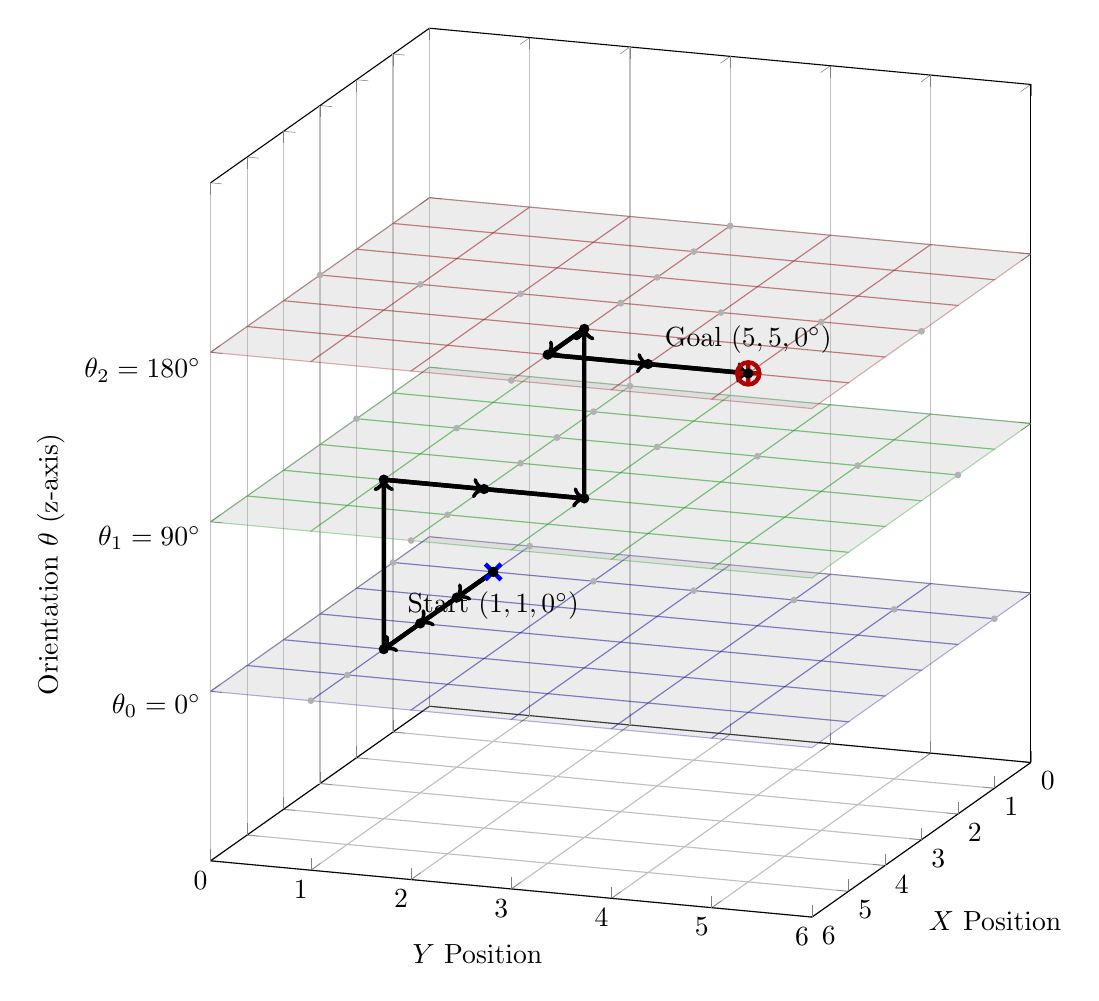
\begin{tikzpicture}
    \begin{axis}[
        view={110}{20},            % Adjust 3D perspective (azimuth, elevation)
        width=12cm, height=10cm,
        xmin=0, xmax=6,
        ymin=0, ymax=6,
        zmin=0, zmax=4,
        xtick={0,1,2,3,4,5,6},
        ytick={0,1,2,3,4,5,6},
        ztick={1,2,3},
        zticklabels={$\theta_0=0^\circ$, $\theta_1=90^\circ$, $\theta_2=180^\circ$},
        xlabel=$X$ Position,
        ylabel=$Y$ Position,
        zlabel=Orientation $\theta$ (z-axis),
        grid=major,
        z buffer=sort,             % Ensures correct layering in 3D
        z post scale=1.5,          % Stretch the z-axis for clarity
        scatter/use mapped color={draw=mapped color, fill=mapped color},
    ]

    % --- 1. Draw the Stacked Grid Layers ---
    \foreach \z in {1,2,3} {
        \addplot3 [
            only marks,
            mark=*,
            mark size=1pt,
            fill=black!30,
            draw=black!30,
        ] coordinates {
            (0,\z, \z) (1,\z, \z) (2,\z, \z) (3,\z, \z) (4,\z, \z) (5,\z, \z) (6,\z, \z)
            (\z,0, \z) (\z,1, \z) (\z,2, \z) (\z,3, \z) (\z,4, \z) (\z,5, \z) (\z,6, \z)
            % (Generate a 7x7 grid for each layer)
        };
        % Simplified grid generation for each layer
        % \addplot3 [mesh, lightgray, opacity=0.3] coordinates {
        %     (0,0,\z) (6,0,\z) (6,6,\z) (0,6,\z) (0,0,\z)
        %     (1,0,\z) (1,6,\z)
        %     (2,0,\z) (2,6,\z)
        %     (3,0,\z) (3,6,\z)
        %     (4,0,\z) (4,6,\z)
        %     (5,0,\z) (5,6,\z)
        %     (0,1,\z) (6,1,\z)
        %     (0,2,\z) (6,2,\z)
        %     (0,3,\z) (6,3,\z)
        %     (0,4,\z) (6,4,\z)
        %     (0,5,\z) (6,5,\z)
        % };

        \addplot3 [surf, samples=7, samples y=7,
                    domain=0:6,domain y=0:6, lightgray, opacity=0.3] {
            \z
        };
    }

    % --- 2. Define and Mark Start and Goal ---
    \node[label={below:Start $(1,1,0^\circ)$}] (start) at (axis cs:1,1,1) {};
    \addplot3[only marks, mark=x, mark size=4pt, draw=blue, ultra thick] coordinates {(1,1,1)};

    \node[label={above:Goal $(5,5,0^\circ)$}] (goal) at (axis cs:5,5,3) {};
    \addplot3[only marks, mark=oplus, mark size=4pt, draw=red!70!black, ultra thick] coordinates {(5,5,3)};

    % --- 3. Visualize State Transitions (Primitives) ---
    % We show example transitions (Reeds-Shepp or similar primitives)

    % Transitions from (1,1,0°) [Layer 1]
    \draw[->, gray, thin, dashed] (axis cs:1,1,1) -- (axis cs:2,1,1);     % Straight
    % \draw[->, gray, thin, dashed] (axis cs:1,1,1) -- (axis cs:2,2,2);     % Turn Left +90°
    % \draw[->, gray, thin, dashed] (axis cs:1,1,1) -- (axis cs:2,0,4);     % Turn Right -90° (wraps to z=4 but not plotted)

    % Transitions along the eventual path (e.g., in Layer 1)
    \draw[->, gray, thin] (axis cs:2,1,1) -- (axis cs:3,1,1);
    \draw[->, gray, thin] (axis cs:3,1,1) -- (axis cs:4,1,1);

    % Inter-layer transition example (Change theta)
    \draw[->, teal, ultra thick] (axis cs:4,1,1) -- (axis cs:4,1,2);       % Rotate to 90° (Layer 2)
    \draw[->, gray, thin] (axis cs:4,1,2) -- (axis cs:4,2,2);             % Straight in Layer 2
    \draw[->, gray, thin] (axis cs:4,2,2) -- (axis cs:4,3,2);

    % Transition from Layer 2 to Layer 3
    \draw[->, purple, ultra thick] (axis cs:4,3,2) -- (axis cs:4,3,3);     % Rotate to 180° (Layer 3)
    \draw[->, gray, thin] (axis cs:4,3,3) -- (axis cs:5,3,3);             % Straight in Layer 3

    % --- 4. Visualize the A* Path ---
    % We define the path from Start (1,1,1) to Goal (5,5,3)
    \addplot3 [
        ultra thick,
        color=mapped color,
        mark=*,
        mark size=1pt,
    ] coordinates {
        (1,1,1)
        (2,1,1)
        (3,1,1)
        (4,1,1) % Transition point: change z (theta)
        (4,1,2)
        (4,2,2)
        (4,3,2) % Transition point: change z (theta)
        (4,3,3)
        (5,3,3)
        (5,4,3)
        (5,5,3)
    };

    % Draw connections for the path in color
    \draw[->, mapped color, ultra thick] (axis cs:1,1,1) -- (axis cs:2,1,1);
    \draw[->, mapped color, ultra thick] (axis cs:2,1,1) -- (axis cs:3,1,1);
    \draw[->, mapped color, ultra thick] (axis cs:3,1,1) -- (axis cs:4,1,1);

    % Colored vertical transitions
    \draw[->, mapped color!80!black, ultra thick] (axis cs:4,1,1) -- (axis cs:4,1,2);
    \draw[->, mapped color!80!black, ultra thick] (axis cs:4,3,2) -- (axis cs:4,3,3);

    % Connections in other layers
    \draw[->, mapped color, ultra thick] (axis cs:4,1,2) -- (axis cs:4,2,2);
    \draw[->, mapped color, ultra thick] (axis cs:4,2,2) -- (axis cs:4,3,2);
    \draw[->, mapped color, ultra thick] (axis cs:4,3,3) -- (axis cs:5,3,3);
    \draw[->, mapped color, ultra thick] (axis cs:5,3,3) -- (axis cs:5,4,3);
    \draw[->, mapped color, ultra thick] (axis cs:5,4,3) -- (axis cs:5,5,3);

    \end{axis}
\end{tikzpicture}
\end{document}